% Unofficial University of Edinburgh
% https://github.com/andiac/gemini-cam
% a fork of https://github.com/anishathalye/gemini
% also refer to https://github.com/k4rtik/uchicago-poster
% Adapted from the University of Cambridge Version

\documentclass[final]{beamer} 

% ====================
% Packages
% ====================

\usepackage[T1]{fontenc}
\usepackage{lmodern}
%\usepackage[size=custom,width=120,height=72,scale=1.0]{beamerposter}
\usepackage[size=custom,width=120,height=72,scale=1.15]{beamerposter}
%\usepackage[orientation=landscape,size=a1,scale=1.4]{beamerposter}
%\usepackage[size=custom,width=108,height=63,scale=1]{beamerposter}
\usetheme{gemini}
\usecolortheme{customuoe}
\usepackage{graphicx}
\usepackage{booktabs}
\usepackage{tikz}
\usepackage{pgfplots}
\pgfplotsset{compat=1.14}
\usepackage{anyfontsize}
\usepackage{multicol}
\usepackage{listings}
\usepackage{color}

\definecolor{dkgreen}{rgb}{0,0.6,0}
\definecolor{grey}{rgb}{0.5,0.5,0.5}
\definecolor{mauve}{rgb}{0.58,0,0.82}

\lstset{frame=tb,
  language=Python,
  aboveskip=3mm,
  belowskip=3mm,
  showstringspaces=false,
  columns=flexible,
  basicstyle={\small\ttfamily},
  numbers=none,
  numberstyle=\tiny\color{grey},
  keywordstyle=\color{dkgreen},
  commentstyle=\color{grey},
  stringstyle=\color{red},
  breaklines=true,
  breakatwhitespace=true,
  tabsize=3,
  frame=none
}

% ====================
% apparently listings and verbatim envionments don't like working inside blocks so this is maybe needed??
% ====================

\newenvironment{code}{\verb|}

\newcommand{\ind}{\phantom{aaa}}

% ====================
% Lengths
% ====================

% If you have N columns, choose \sepwidth and \colwidth such that
% (N+1)*\sepwidth + N*\colwidth = \paperwidth
\newlength{\sepwidth}
\newlength{\colwidth}
\setlength{\sepwidth}{0.025\paperwidth}
\setlength{\colwidth}{0.3\paperwidth}

\newcommand{\separatorcolumn}{\begin{column}{\sepwidth}\end{column}}

% ====================
% Title
% ====================

\title{Projective Geometry and Dobble}

\author{Ben Jecock, Corinne Bernard, Eric Rogers, Samuel Buxton, Teagan Addy}

% ====================
% Footer (optional)
% ====================

%\footercontent{
%  \href{https://www.example.com}{https://www.example.com} \hfill
%  ABC Conference 2025, New York --- XYZ-1234 \hfill
%  \href{mailto:alyssa.p.hacker@example.com}{alyssa.p.hacker@example.com}}
% (can be left out to remove footer)

% ====================
% Logo (optional)
% ====================

% use this to include logos on the left and/or right side of the header:
% \logoright{\includegraphics[height=7cm]{logo1.pdf}}
%\logoleft{
\includegraphics[height=7cm]{logos/uoelogo.png}}

\setbeamertemplate{bibliography entry article}{}
\setbeamertemplate{bibliography entry title}{}
\setbeamertemplate{bibliography entry location}{}
\setbeamertemplate{bibliography entry note}{}

% ====================
% Body
% ====================

\begin{document}

% Refer to https://github.com/k4rtik/uchicago-poster
% logo: https://www.cam.ac.uk/brand-resources/about-the-logo/logo-downloads
\addtobeamertemplate{headline}{}
{
    \begin{tikzpicture}[remember picture,overlay]
      \node [anchor=north west, inner sep=3cm] at ([xshift=-1.0cm,yshift=1.0cm]current page.north west)
      {
\includegraphics[height=4.5cm]{logos/uoelogo.png}}; 
    \end{tikzpicture}
}

\begin{frame}[t]
\begin{columns}[t]
\separatorcolumn

\begin{column}{\colwidth}

  \begin{block}{Introduction}
    Dobble is a game created by Jacques Cottereau - a French mathematics enthusiast. Cottereau’s idea for the game came from a fascination for combinatorics, pairs and ordering and is said to be inspired by Kirkman’s schoolgirl problem. There are $55$ cards in a standard game of Dobble, each containing $8$ distinct symbols from a pool of $57$ unique symbols. The game has taken many different forms - some versions aim to get rid of your cards first, some to collect as many as possible, or even to sabotage your opponents. However, the key principle of the game is that every unique pair of Dobble cards contains one symbol in common. Although this fact seems like a coincidence, it relies on aspects of geometry, combinatorics, the projective - and finite projective - plane. 
  \end{block}

  \begin{alertblock}{The Dobble Problem and Combinatorics}

    Let us first imagine that we have a big set $A$ of unique items. We wish to create subsets of $A$ which contain a fixed, equal number of items within them.
    
    The rule is that these subsets have to have an overlap of \emph{one item} - there cannot be an overlap of two unique items between any two subsets. In effect, for any pair of items in any subset, \emph{this pair cannot reappear in any other subset}.

    This is known as a Steiner system notated as $S(2,k,n)$, where $k$ is the number of subsets (known as blocks) and $n$ is the number of total items. (It can also be referred to as a symmetric $2$-design, a $2$-$(n,k,1)$ design).

This problem is very much akin to Dobble - in essence, the items are points and the subsets/blocks are cards. For the standard version of Dobble, we essentially just have the Steiner system $S(2,8,57)$.
These parameters are because:
\begin{itemize}
    \item We have $57$ cards total in Dobble
    \item There are cards (blocks) with $8$ symbols with the constraint that
    \item Any pair of $2$ pictures are contained in \emph{exactly} one card (block).
\end{itemize}

However, there exists a link between Steiner systems and projective planes. If we have a finite projective plane $P$ such that any line has exactly $q+1$ points, we can conclude that there are $q^2+q+1$ total points in $P$, and that $P$ is a $S(2, q+ 1, q^2 +q+ 1)$
Steiner system (or a $2$-$(q^2 +q+ 1, q + 1, 1)$ design) \cite{storme2006}.
  \end{alertblock}
  
  \begin{block}{Finite Fields}

      A field is a set where arithmetic behaves in accordance with the field axioms \cite{Weisstein2023b}. Field axioms are a set of properties a field is required to have. These can be written in additive and multiplicative pairs. These pairs are associativity, commutativity, distributivity, identity and inverse \cite{Weisstein2023}. It is then rather intuitive that a finite field is thus a finite set of elements that satisfy these properties. The number of elements within a finite field is referred to as its order. A finite field can only exist if it has order $q=p^k$ where $p$ is a prime number and $k\in\mathbb{Z}^+$ \cite{cameron2000} (this is denoted as $\mathbb{F}_q$). This is to say that the order of a finite field can only be prime, or a power of a prime number \cite{cameron2000}. Using a finite field we can build a vector space, and its associated projective plane is a \emph{finite} projective plane. A finite field of order $q=p^k$ will produce the projective plane with $q^2+q+1$ points and lines \cite{Collingridge2018}.

  \end{block}

\end{column}

\separatorcolumn

\begin{column}{\colwidth}

\begin{block}{Steiner Systems, Dobble and Projective Planes}

    Consider a game of Dobble with only $7$ cards. If each point represents a card, lines can be drawn such that if we were to chose any two of the seven points there is a line that connects them. We can say that these lines represent matching symbols on each card. 

     So, if we draw this configuration for the $7$ card example we get the Fano Plane, shown in Figure \ref{fig:fano}.
    \begin{multicols}{2}
\begin{figure}
      \centering
      \begin{tikzpicture}[scale=3]
  \draw \foreach \a in {30,150,270}{(\a:1)  -- (180+\a:2)}
        (90:2)  -- (210:2) -- (330:2) -- cycle
        (0:0) circle (1);
  \fill \foreach \p in {(0:0),(30:1),(90:2),(150:1),(210:2),(270:1),(330:2)}
        {\p circle(3pt)};
        \end{tikzpicture}
      \caption{7 Card Dobble - The Fano Plane}
      \label{fig:fano}
\end{figure}

\begin{figure}
    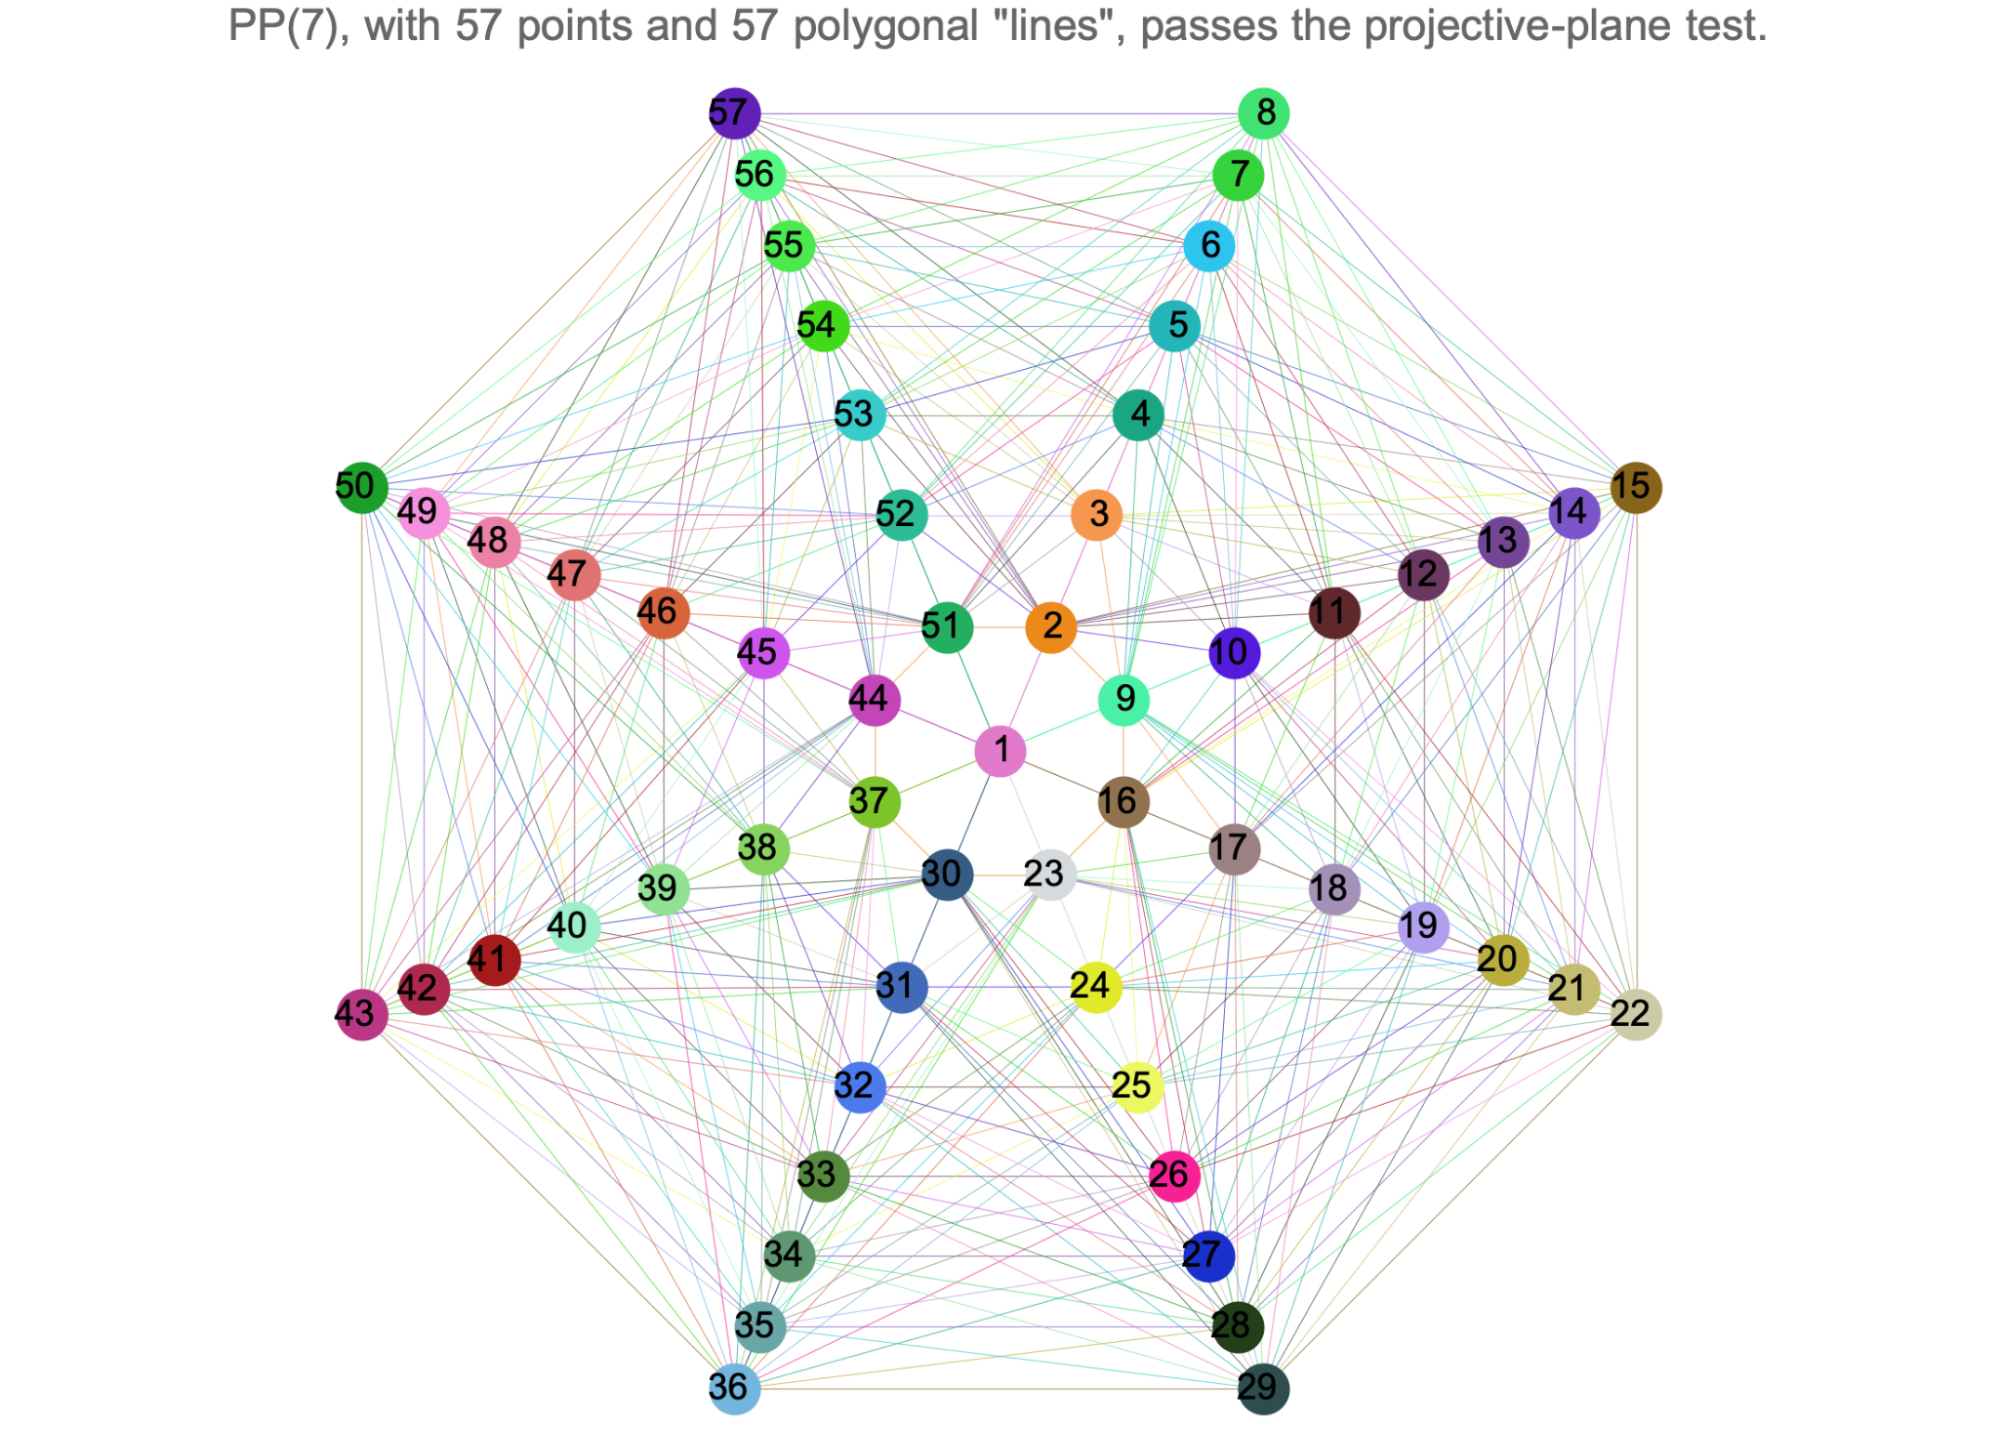
\includegraphics[width=14cm,trim={0 0.5cm 0 2cm},clip]{image1}
    \caption{57 Cards - The Finite Plane (order 7) \cite{beresford2011}}
    \label{fig:pporder7}
\end{figure}
    \end{multicols}
  
    It follows that each card contains $3$ symbols, no two cards are the same (i.e. no lines are parallel) and any two cards will have one and \emph{only one} matching symbol with $7$ different symbols in total \cite{westenbrink2022}.
    We can see that this is just the Steiner system $S(2,3,7)$ where $q = p^n = 2^1$, $q + 1 = 3$ (no. of symbols on each card) and $q^2 + q + 1 = 7$, which is the no. of cards and the total no. of symbols.
    
    Now we can apply this to our full sized version of Dobble. We can start by constructing a $7\times7$ grid of points and lines such that if we choose any two of the $49$ points there is a line that connects them. This can be achieved by ''Wrapping around`` the grid until it goes through $7$ points. This grid can be seen in Figure \ref{fig:pporder7}.

    We are then left with a grid of $56$ lines and we can see that there are actually $8$ different systems of $7$ parallel lines. Each collection of parallel lines converges at infinity at some point \cite{spencer1999}, hence there are $8$ more points at infinity that can be connected with a final line. Therefore, all lines (now $57$ in total) go through $8$ points \cite{Parker2021}.

    This can also be framed as a representation of $S(2,8,57)$ where $q = p^n = 7^1$, $q + 1 = 8$ (no. of symbols on each card) and $q^2 + q + 1 = 57$, the no. of cards and the total no. of symbols. 

    It is theorised that to simplify the printing process there are only $55$ cards in Dobble. Cards can still be arranged in the same way, essentially `skipping' these points and the game will still work. 

\end{block}

\begin{exampleblock}{Generating Dobble Decks}

    The key to representing a game of Dobble as a finite projective plane of a prime power order $q = p^n$, is to find the set $S$ of all elements in $\mathbb{F}_q$: three-tuples $[a:b:c]$ where $[a:b:c] \equiv [\lambda a:\lambda b:\lambda c] \mod p$ for $a,b,c,\lambda \in \mathbb{F}_q, \lambda \ne 0$. When $n = 1$, i.e. $q$ is prime, we have $S = \{0, 1, ... q-1\}$. 
\end{exampleblock}
\end{column}

\separatorcolumn

\begin{column}{\colwidth}
\begin{exampleblock}{Generating Dobble Decks (cont.)}
    However, if $n > 1$, the corresponding set $\{ 0, 1, ... p^n-1 \}$ equipped with the operators $+$ and $\times$ modulo $p$ is not a field; we can instead construct a finite field of degree $p^n$ by using a polynomial basis. This is the set $S$ of all polynomials such that $c_0 + c_1x + c_2x^2 + \cdots + c_{n-1}x^{n-1}$ where $c_0, ..., c_{n-1} \in \{0, 1, ... p-1\}$, and we also require an irreducible polynomial over $S$ of degree $n$ for the first modulus of the polynomial addition and multiplication operations (then we also work modulo $p$); such an irreducible polynomial always exists \cite{magidin2012}.
    
    Once we have the set of all elements in $\mathbb{P}^2_{\mathbb{F}_q}$, we can use the property of the duality of finite projective planes: any statement is equally valid if the points and lines are exchanged. Hence, we can interpret the points also as lines, and if the sum of the corresponding components of a point and a line multiplied equals zero, then that point (symbol) lies on that line (card).

    As an example, we shall look at the process of generating a deck for $q = 3^2$:

    \begin{enumerate}
        \item Find the set $S$ of elements in the finite field $\mathbb{F}_9$ (its basis):
            \begin{equation*}
                S = \left\{ \sum_{i=0}^{2-1} c_ix^i : c_i \in \mathbb{Z}^+, c_i < 3 \right\} = \left\{ 0, 1, 2, x, x+1, x+2, 2x, 2x+1, 2x+2 \right\}
            \end{equation*}
        \item Find an irreducible polynomial $g(x)$ of degree $n = 2$. We do this by exhaustion (note that for $n=1$, $x$ is irreducible by definition). We find that $g(x) = x^2+1$ is irreducible over $S$.
        \item find the set of all elements in the finite field $\mathbb{P}^2_{\mathbb{F}_9}$ (avoiding counting $[a:b:c]$ and $[\lambda a:\lambda b:\lambda c]$ as they are equivalent). We do this by counting them as

        \begin{center}
            \begin{minipage}{14em}
                \lstinputlisting{code_example.py}
            \end{minipage}
        \end{center}

        \item Find which points are incident to which lines (using the property of duality). We shall treat the three-tuples in $\mathbb{P}^2_{\mathbb{F}_9}$ as vectors in $\mathbb{R}^3$: the incidences of the points and lines are then given for a position vector $P = \langle a,b,c \rangle$ and a line $\ell = \langle 0,0,0 \rangle + \mu \langle \alpha,\beta,\gamma \rangle$ such that $P \cdot \ell = 0 \mod g(x) \mod p$.

        \item The combinations of points on each line is analogous to the combinations of symbols on cards: we have $q+1$ symbols on each of the $q^2+q+1$ cards.
    \end{enumerate}

  \end{exampleblock}

 
  \begin{block}{References}
%   \nocite{*}
    \vspace{-0.25em}
\footnotesize{\bibliographystyle{unsrt}\bibliography{poster}}
  \end{block}

\end{column}

\separatorcolumn
\end{columns}
\end{frame}

\end{document}
